\newpage % Rozdziały zaczynamy od nowej strony.
\section{Przeglad }
W rozdziale tym dokonuje przeglądu istotnych zagadnień związanych z zarządzaniem łańcuchem dostaw oraz uczeniem maszynowym. Przedstawimy definicje, teorie, rodzaje  zarządzania łańcuchem dostaw  i maszynowego uczenia . Następnie omówiam definicje i zastosowania maszynowego uczenia w zarządzaniu łańcuchem dostaw.


\subsection{Zarządzania łańcuchem dostaw}
W niniejszym podrozdziale dokładnie omówiam najważniejsze zagadnienia związane z zarządzaniem łańcuchem dostaw( definicje, cele oraz znaczenie) . Ponadto wyjaśniam z jakich elementów składa się zarządzanie łańcuchem dostaw.

\vspace{\baselineskip}
\subsubsection{Definicje Zarządzania Łańcuchem Dostaw} 
\vspace{\baselineskip}
\textbf{Definicje z różnych źródeł:}

Zarządzanie łańcuchem dostaw (ang. Supply Chain Management, SCM) jest kompleksowym podejściem do planowania, kontrolowania i monitorowania wszystkich procesów związanych z dostarczaniem produktów lub usług od dostawców do klientów końcowych. Jest to obszar, który obejmuje wiele etapów, począwszy od zaopatrzenia, produkcji, dystrybucji, aż po dostarczenie produktu lub usługi do ostatecznego użytkownika.

Zarządzanie łańcuchem dostaw (ang. Supply Chain Management – SCM) – zarządzanie przepływami między ogniwami łańcuchem dostaw. Umożliwia projektowanie, planowanie, realizację, kontrolę oraz monitoring łańcucha dostaw. \cite{wik2023}



Wg. Encyklopedii zarzadzania Łańcuch dostaw - obejmuje wszelkie czynności związane z transportem oraz przeróbką towarów, wspominając tutaj również o początkowym etapie, czyli pozyskiwaniu wszelkiego rodzaju surowców oraz etapie końcowym tj. dostarczeniu produktu konsumentom. Pojęcie to zawiera również przepływ informacji, które są istotne podczas całego procesu. \cite{zarz2023}

Zarządzanie łańcuchem dostaw obejmuje wszystkie działania, które przekształcają surowce w gotowe produkty i oddają je w ręce klientów. Może to obejmować określanie źródła dostaw, projektowanie, produkcję, magazynowanie, wysyłkę i dystrybucję. Celem SCM jest poprawa wydajności, jakości, produktywności i zadowolenia klientów. \cite{scm2023}

Łańcuch dostaw jest to skoordynowana sieć wzajemnych powiązań logistyczno - operacyjnych, która obejmuje wszelkie firmy, obiekty i działania biznesowe zaangażowane w pozyskiwanie, opracowywanie, wytwarzanie i dostarczanie produktów.
Każda firma tworzy swój własny łańcuch dostaw, aby móc wytwarzać produkty i wprowadzać je na rynek. Może również sama być ogniwem w łańcuchach dostaw innych firm. Działania łańcucha dostaw przekształcają zasoby naturalne, surowce i komponenty w gotowy produkt, który jest dostarczany do użytkownika końcowego. \cite{wdx2023}

 (SCM) zajmuje się systemem zakupów (zakup surowców/komponentów), zarządzaniem operacyjnym (zapewnienie produkcji wysokiej jakości produktów z dużą szybkością, dobrą elastycznością i niskimi kosztami produkcji), logistyką i kanałami marketingowymi , dzięki któremu surowce można przekształcić w gotowe produkty i dostarczyć klientom końcowym.Węższa definicja zarządzania łańcuchem dostaw to „projektowanie, planowanie, realizacja, kontrola i monitorowanie działań w łańcuchu dostaw w celu tworzenia wartości netto, budowania konkurencyjnej infrastruktury, wykorzystania światowej logistyki, synchronizacji podaży z popytem i pomiaru wydajności globalnie”. Może to obejmować przemieszczanie i przechowywanie surowców, zapasów w toku, wyrobów gotowych i kompleksową realizację zamówień od punktu pochodzenia do punktu konsumpcji. \cite{wiken2023}

\vspace{\baselineskip}
\textbf{Historia}
Łańcuchy dostaw istnieją od czasów starożytnych, poczynając od pierwszego wytworzonego i sprzedanego produktu. Wraz z nadejściem industrializacji zarządzanie łańcuchem dostaw stało się bardziej złożone i pozwoliło przedsiębiorstwom na efektywniejsze wytwarzanie i dostarczanie towarów i usług. Na przykład wprowadzona przez Henry'ego Forda standaryzacja części samochodowych okazała się przełomem, który pozwolił na masową produkcję towarów, aby sprostać wymaganiom rosnącej liczby klientów. Z biegiem czasu kolejne zmiany (takie jak wprowadzenie na rynek komputerów) systematycznie zwiększały poziom zaawansowania systemów SCM. Systemy te pozostawały jednak przez wiele lat zasadniczo liniową, autonomiczną funkcją zarządzaną przez specjalistów ds. łańcucha dostaw. 
Sytuacja zmieniła się diametralnie wraz z pojawieniem się Internetu, innowacji technologicznych i gospodarki globalnej opartej na popycie. Obecnie zarządzanie łańcuchem dostaw nie jest już funkcją liniową, ale raczej złożonym zbiorem niejednorodnych sieci dostępnych całodobowo. W centrum tych sieci znajdują się konsumenci oczekujący realizacji swoich zamówień w wybrany przez nich sposób.\cite{oracle2023}

\vspace{\baselineskip}
\textbf{Pochodzenie terminu}.W 1982 roku Keith Oliver, konsultant w firmie Booz Allen Hamilton, w wywiadzie dla Financial Times wprowadził do domeny publicznej termin „zarządzanie łańcuchem dostaw”. W 1983 roku WirtschaftsWoche w Niemczech opublikowało po raz pierwszy wyniki wdrożonego tzw. „projektu zarządzania łańcuchem dostaw”, kierowanego przez Wolfganga Partscha.
W połowie lat 90. termin „zarządzanie łańcuchem dostaw” zyskał na popularności, gdy ukazała się lawina artykułów i książek na ten temat. Pierwotnie łańcuchy dostaw zdefiniowano jako obejmujące wszystkie działania związane z przepływem i przetwarzaniem towarów od surowców do użytkownika końcowego lub konsumenta końcowego, a także powiązane przepływy informacji. Mentzer i in. uważają za godne odnotowania, że te wcześniejsze definicje obejmowały konsumenta końcowego. Zarządzanie łańcuchem dostaw zostało następnie zdefiniowane jako integracja działań w łańcuchu dostaw poprzez ulepszone relacje w łańcuchu dostaw w celu osiągnięcia przewagi konkurencyjnej. \cite{wiken2023}


\vspace{\baselineskip}
\subsubsection{Cele Zarządzania Łańcuchem Dostaw}



Najczęściej opisywanymi celami łańcucha dostaw w ujęciu logistycznym jest:

  \par - Minimalizacja kosztów wynikających z przepływu towarów i informacji przy zachowaniu dobrego poziomu obsługi klienta
  \par - Krótki czas realizacji zamówień oraz bezproblemowość i elastyczność dostaw
   \par- Optymalizacja poziomu zapasów wraz z dostosowaniem się do potrzeb rynku \cite{zarz2023}


Podsumowujac: Głównym celem zarządzania łańcuchem dostaw jest zapewnienie, że produkty lub usługi są dostarczane w odpowiednim czasie, w optymalnych ilościach, przy minimalnych kosztach oraz z zachowaniem wysokiej jakości. SCM dąży do zintegrowania wszystkich elementów łańcucha dostaw, tak aby procesy były bardziej efektywne i konkurencyjne.

Ale wazne aby odnotować zmiane w celach ..raczej ktore cele sa obecnie najwazniejsze:
Dzisiejsze systemy SCM są całkowicie ukierunkowane na klienta
Celem zarządzania łańcuchem dostaw zawsze było zwiększanie efektywności i obniżanie kosztów. Cele te nie uległy zmianie, ale obecnie główną rolę w ustalaniu priorytetów takiego zarządzania odgrywa klient. Mówi się, że „doświadczenia klientów żyją i umierają w łańcuchu dostaw”.
Lojalność klientów zależy od tego, czy przedsiębiorstwo jest w stanie szybko i dokładnie spełnić ich oczekiwania. Dostawy surowców, produkcja, logistyka, sprzedaż i zarządzanie zamówieniami muszą być ze sobą skoordynowane, aby klient otrzymał to, co chce, w rozsądnym terminie. W tym celu przedsiębiorstwo musi analizować swoje łańcuchy dostaw z perspektywy klientów. Nie chodzi tu bowiem tylko o terminową dostawę, ale również o wykonanie we właściwym czasie wszystkich niezbędnych czynności, zarówno przed taką dostawą, jak i w jej trakcie oraz po jej zrealizowaniu.\cite{oracle2023}


\vspace{\baselineskip}
\subsubsection{Znaczenie zarządzania Łańcuchem Dostaw}

Łańcuchy dostaw zawsze były napędzane przez wiele sił globalnych i politycznych, a nawet przez warunki pogodowe i wydarzenia naturalne. Jest jednak jedna rzecz, która jest pewna w zarządzaniu łańcuchem dostaw i to jest zmiana. 
Nowoczesna logistyka stawia menedżerów przed wieloma wyzwaniami skutecznej organizacji łańcuchów dostaw, optymalizacji kosztów i zarządzania stanami magazynowymi. Wszystko to ułatwią rozwijające się technologie Łańcuchów Dostaw 4.0. To szerokie pojęcie obejmuje między innymi zastosowanie IoT w logistyce, użycie zaawansowanej robotyki w magazynach oraz zaawansowaną analizę Big Data, a nawet sztuczną inteligencję. Dzięki czujnikom, sieciom, nowoczesnemu oprogramowaniu i automatyzacji możliwe jest nie tylko zwiększenie skuteczności procesów logistycznych, ale także ograniczenie kosztów oraz wyższy poziom zadowolenia klienta z dostaw.
Znaczenie systemów SCM: Istota zarządzania łańcuchem dostaw
Wystarczy się rozejrzeć. Wszystko, co znajduje się w Twoim domu lub zakładzie pracy, trafiło tu dzięki łańcuchom dostaw. Działania te wymagają zaangażowania pracowników z milionów miejsc pracy na całym świecie. Przez łańcuch dostaw przewija się wszystko — od tanich dóbr konsumpcyjnych aż po przyrządy chirurgiczne i kluczowe zasoby. Wciąż jednak, mimo iż zarządzanie łańcuchami dostaw leży u podstaw gospodarki światowej, wiele organizacji korzysta w tym celu z procesów i maszyn stosowanych od 50 lat.\cite{scm2023}

  Wiele firm po prostu przestałoby działać bez zarządzania łańcuchem dostaw, więc to dość duże korzyści SCM.  Niektóre z zalet zoptymalizowanego zarządzania łańcuchem dostaw obejmują: 

   - Większa produktywność: systemy do zarządzania zasobami przedsiębiorstwa i przeglądy zapobiegawcze zwiększają wydajność maszyn i systemów. Może to pomóc w wyeliminowaniu wąskich gardeł, usprawnieniu procesów i zwiększeniu produktywności. Zautomatyzowane procesy i responsywne analizy danych przekładają się na szybszy transport i krótszy czas dostawy.
   
   -Niższe koszty łańcucha dostaw: przy użyciu analiz predykcyjnych można wyeliminować konieczność szacowania w oparciu o przypuszczenia. Pozwoli to ograniczyć zarówno marnotrawienie zapasów, jak i ryzyko ich deficytu. Internet rzeczy zapewnia większą responsywność istniejących zasobów oraz maksymalnie wydajny i praktyczny przepływ pracy w każdej sytuacji. Bardziej precyzyjne prognozy umożliwiają ponadto redukcję liczby niezaładowanych w pełni samochodów dostawczych i nieskoordynowanych tras dostaw, a także bardziej efektywne zarządzanie flotą.
   
   - Większa elastyczność i odporność łańcucha dostaw: Trendy i zmiany na rynku mogą nastąpić nagle. Odporne systemy SCM są elastyczne, aby dostosować się do każdej sytuacji. Dane w czasie rzeczywistym i inteligentne analizy mogą pomóc menedżerom łańcucha dostaw przenieść maszyny i personel do lepszych przepływów pracy. Opinie klientów można od razu usłyszeć i podjąć odpowiednie działania. Wirtualne zapasy i inteligentne procesy magazynowe zapewniają dostosowanie podaży i popytu.
   
   -Wyższa jakość produktów: zapewnienie zespołom ds. badań i rozwoju dostępu do informacji zwrotnych od klientów sprawia, że podczas projektowania i opracowywania produktów brane są pod uwagę ich potrzeby. Zarówno zespół ds. badań i rozwoju, jak i zespół ds. produkcji mogą wykorzystać informacje dostępne dzięki uczeniu maszynowemu i analizom, aby reagować na trendy i oczekiwania klientów oraz doskonalić projekty produktów.
    
    -Lepsza obsługa klienta: najlepsze praktyki SCM są zorientowane na klienta i zaprojektowane tak, aby były responsywne i adaptacyjne. Dzięki konkurencji tylko jednym kliknięciem, nowoczesny SCM pozwala firmom wdrażać opinie klientów i trendy, umożliwiając zarówno mikrorealizację, jak i personalizację na dużą skalę.
    
    -Większa przejrzystość i zrównoważony rozwój: SCM umożliwia pełną przejrzystość, od etapu projektowania i produkcji po logistykę, dostawę i zwroty. Dzięki możliwości wglądu we wszystkie dane wejściowe i wyjściowe w całym łańcuchu organizacje mogą znacznie poprawić swój wpływ na środowisko, często współpracując w tym celu bezpośrednio z dostawcami i innymi dostawcami. \cite{scm2023}

 

\vspace{\baselineskip}
\subsubsection{Składniki Efektywnego Zarządzania Łańcuchem Dostaw}



Elementy łańcucha dostaw

Istnieje pięć elementów tradycyjnych systemów zarządzania łańcuchem dostaw:

    -Planowanie. Planowanie i zarządzanie wszystkimi zasobami wymaganymi do zaspokojenia zapotrzebowania klientów na produkt lub usługę firmy. Po ustanowieniu łańcucha dostaw należy określić mierniki, które pozwolą zmierzyć czy łańcuch dostaw jest wydajny, efektywny, zapewnia wartość klientom i spełnia cele firmy.
    
   - Zaopatrzenie. Wybór dostawców kwalifikowanych, którzy zapewnią towary i usługi potrzebne do stworzenia produktu. Należy również ustalić procesy monitorowania i zarządzania relacjami z dostawcami. Kluczowe działania w tych procesach obejmują zamawianie, przyjmowanie, zarządzanie stanami magazynowymi oraz realizację płatności dla dostawców.
    
   - Produkcja. Czynności wymagane do przyjęcia surowców, wytworzenia produktu, badania jakości, opakowania do wysyłki i przygotowania harmonogramu dostaw.
    
   - Dostawa i logistyka. Koordynacja zamówień klientów, magazynowanie, planowanie dostaw, wysyłka towarów, wystawianie faktur i odbieranie płatności.
    
   - Zwroty. Stworzenie procesu odbioru wadliwych, nadmiarowych lub niechcianych produktów\cite{wdx2023}



Aleksander Wielki powiedział kiedyś słynnie: „Moi logistycy nie mają poczucia humoru… ponieważ wiedzą, że jeśli moja kampania się nie powiedzie, są pierwszymi, których zabiję”. I choć ten przykład jest trochę skrajny, niemniej jednak ilustruje on, jak ważne dla cywilizacji ludzkiej były zawsze łańcuchy dostaw. Efektywne i odporne narzędzia i praktyki w zakresie zarządzania łańcuchem dostaw są niezbędnym elementem przetrwania i sukcesu firmy. Niektóre z podstawowych procesów SCM obejmują:   

    -Planowanie łańcucha dostaw to proces przewidywania popytu na produkty i koordynowania powiązań w łańcuchu dostaw w celu jego realizacji. Oprócz prognozowania popytu i planowania obejmuje on planowanie dostaw, planowanie potrzeb materiałowych (MRP), planowanie produkcji, planowanie sprzedaży i produkcji (SOP)i inne. 

   - Zarządzanie cyklem życia produktu (PLM) to proces zarządzania produktem przez cały jego cykl życia – od ideacji, inżynierii i projektowania po produkcję, serwis i utylizację (lub recykling).

    -Nabycie to proces nabywania materiałów, towarów i usług w celu zaspokojenia potrzeb biznesowych i zapewnienia jakości, uczciwej ceny i wartości tych towarów. Głównym wyzwaniem dla zespołów s. zaopatrzenia i określania źródła dostaw jest przewidywanie dokładnych wolumenów zamówień, ponieważ zarówno niedobory, jak i nadwyżki mogą być szkodliwe dla firmy. 

   - Zarządzanie logistyką to transport i składowanie towarów od początku łańcucha dostaw, z surowcami i produkcją, po dostawę gotowych produktów do sklepów lub klientów – a nawet do obsługi produktów, zwrotów i recyklingu. Funkcje biznesowe obejmują zarządzanie transportemprzychodzącym i wychodzącym, zarządzanie flotą, gospodarkę magazynową, kontrolę zapasów i obsługę klienta. 

   - Zarządzanie realizacją produkcji (MES) monitoruje, śledzi, dokumentuje i kontroluje proces wytwarzania towarów. Utrzymuje produkcję i procesy tak szczupłe, jak to tylko możliwe – zachowując (i poprawiając) jakość, zrównoważony rozwój i zadowolenie klientów. 

   - Zarządzanie aktywami przedsiębiorstwa to proces zarządzania aktywami fizycznymi i ich utrzymania w całym łańcuchu dostaw, od robotyki fabrycznej po floty dostaw. Czujniki IoT, łączność maszyna-maszyna (M2M)– poprawiają wydajność, czas pracy, bezpieczeństwo oraz prewencyjną i predykcyjną konserwację. Niektóre połączone zasoby mogą nawet przewidywać naprawy lub awarie i samodzielnie przeprowadzać konserwację — bezpośrednio do określania źródła dostaw i zamawiania części potrzebnych do wydłużenia cyklu życia.\cite{scm2023}






\subsection{Maszynowe Uczenie}

W tym rozdziale omawiamy podstawowe koncepcje i techniki związane z maszynowym uczeniem. Rozpoczynamy od wprowadzenia do sztucznej inteligencji, definiując, czym jest i jakie są jej główne komponenty. Następnie skupiamy się na maszynowym uczeniu, jego znaczeniu i zastosowaniach.


\vspace{\baselineskip}
\subsubsection{Sztuczna Inteligencja (SI)}
\textbf
Sztuczna inteligencja to dziedzina informatyki, która zajmuje się tworzeniem systemów komputerowych zdolnych do wykonywania zadań, które normalnie wymagają ludzkiego myślenia. SI składa się z kilku głównych komponentów, obejmujących:

\textbf {Definicje sztucznej inteligencji}
Sztuczna inteligencja jest tematem obszernym i szeroko omawianym zarówno w sferze naukowej, publicystycznej, jak i politycznej. Są to działania oparte o modelowanie wiedzy, danych i rozwijanie systemów algorytmów oraz mocy obliczeniowych, co w obecnym stanie techniki pozwala na uzyskanie względnie zautomatyzowanego systemu pozyskiwania, przetwarzania i analizy danych, który daje możliwość samoistnego (autonomicznego) ulepszania systemu lub przewidywania zachowań i działań na podstawie analizy zebranych danych i korelacji między nimi, z możliwością wpływu na środowisko zewnętrzne oraz pozostające z nim w interakcji za pomocą sensorów i siłowników. Interakcje te mogą zachodzić mechanicznie lub z udziałem człowieka w cyklu życia sztucznej inteligencji począwszy od etapu kreacji, rozwoju, wdrożenia, stosowania, aż po etap decyzji o wyłączeniu z pracy i utylizacji.\cite{gov2023}


Ponizej podział i schemat zastosowan sztucznej inteligencji wg. raportu "Game-changing technologies: Transforming production and employment in Europe"
\begin{figure}[!h]
    \label{fig:ai}
    \centering 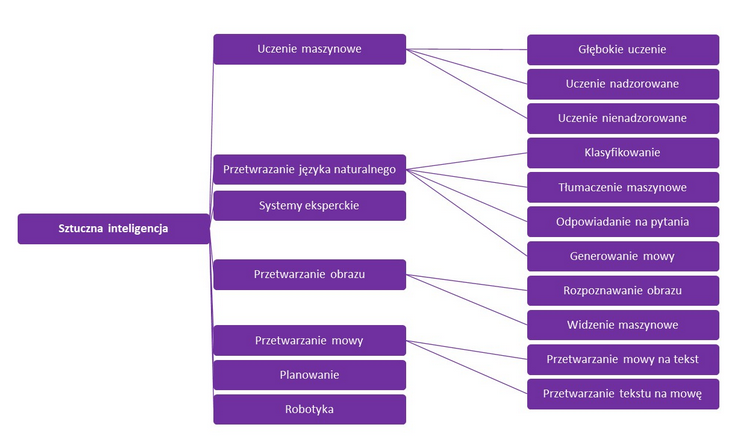
\includegraphics[width=1\linewidth]{AI.png}
    \caption{Obszary zastosowań  sztucznej inteligencji\cite{gov2023}}
\end{figure}

Definicja wg.raportu: "A DEFINITION OF AI:MAIN CAPABILITIES AND DISCIPLINES"  
Sztuczna inteligencja (AI) odnosi się do systemów, które wykazują inteligentne zachowanie poprzez analizę swojego otoczenia i
podejmowanie działań – z pewną dozą autonomii – dla osiągnięcia określonych celów.
Systemy oparte na AI mogą mieć charakter wyłącznie programowy, działać w świecie wirtualnym (np. asystenci głosowi, analiza obrazu
oprogramowanie, wyszukiwarki, systemy rozpoznawania mowy i twarzy) lub sztuczna inteligencja mogą być wbudowane w urządzenia sprzętowe (np.
zaawansowane roboty, samochody autonomiczne, drony czy aplikacje Internetu Rzeczy\cite{ec2029}



\begin{itemize}
    \item \textbf{Uczenie maszynowe (Machine Learning):} Jest to jedna z najważniejszych gałęzi sztucznej inteligencji, która pozwala komputerom na naukę z danych i podejmowanie decyzji na podstawie tych informacji. W ramach uczenia maszynowego wykorzystuje się różne techniki, w tym algorytmy uczenia nadzorowanego i nienadzorowanego.
    
    \item \textbf{Przetwarzanie języka naturalnego (Natural Language Processing - NLP):} Ta dziedzina zajmuje się rozumieniem, przetwarzaniem i generowaniem języka naturalnego przez komputery. NLP jest używane do analizy tekstu, tłumaczenia maszynowego i wielu innych zastosowań.
    
    \item \textbf{Wizja komputerowa:} Obejmuje technologie pozwalające komputerom analizować, rozumieć i interpretować obrazy i wideo. Jest używana w rozpoznawaniu obiektów, rozpoznawaniu twarzy, samochodach autonomicznych i innych dziedzinach.
    
    \item \textbf{Robotyka:} SI jest również istotna w dziedzinie robotyki, gdzie komputery sterują działaniami fizycznymi robotów.
\end{itemize}

\subsubsection{Maszynowe Uczenie}

Maszynowe uczenie (ML) to podzbiór sztucznej inteligencji, który koncentruje się na rozwijaniu algorytmów i technik pozwalających komputerom na naukę z danych i podejmowanie decyzji na podstawie tych informacji. Głównym celem maszynowego uczenia jest rozwijanie modeli, które mogą generalizować zbiory danych i wykonywać zadania bez konieczności programowania ich wprost.

\subsubsection{Zastosowania Maszynowego Uczenia}

Maszynowe uczenie ma szerokie spektrum zastosowań w różnych dziedzinach. W kontekście zarządzania łańcuchem dostaw (SCM), ma to szczególne znaczenie. Poniżej przedstawiamy niektóre z głównych zastosowań ML w SCM:

\begin{itemize}
    \item \textbf{Prognozowanie popytu:} Uczenie maszynowe może być wykorzystywane do prognozowania przyszłego popytu na produkty lub usługi, co pomaga w planowaniu produkcji i zarządzaniu zapasami.
    
    \item \textbf{Optymalizacja zapasów:} Algorytmy ML mogą pomóc w zoptymalizowaniu poziomu zapasów, minimalizując koszty i zapewniając, że dostępność produktów jest na odpowiednim poziomie.
    
    \item \textbf{Wybór dostawcy:} ML może pomóc w analizie dostawców pod kątem efektywności, jakości i kosztów, co ułatwia wybór najlepszego dostawcy.
    
    \item \textbf{Planowanie tras i logistyka:} Algorytmy ML mogą pomóc w optymalizacji tras dostaw, minimalizując czas i koszty transportu.
\end{itemize}

\subsubsection{Rodzaje Maszynowego Uczenia}

Maszynowe uczenie może być podzielone na kilka głównych rodzajów, zależnie od sposobu przetwarzania danych i celu uczenia. Oto niektóre z najważniejszych rodzajów maszynowego uczenia:

\begin{itemize}
    \item \textbf{Uczenie nadzorowane (Supervised Learning):} W tym rodzaju uczenia algorytm jest trenowany na podstawie zestawu danych, który zawiera zarówno wejścia, jak i odpowiadające im oczekiwane wyjścia. Celem jest zbudowanie modelu, który może dokładnie przewidywać wyjście na podstawie nowych danych wejściowych. Przykłady obejmują algorytmy regresji liniowej i klasyfikacji.

    \item \textbf{Uczenie nienadzorowane (Unsupervised Learning):} W przypadku uczenia nienadzorowanego algorytm jest trenowany na danych wejściowych bez oczekiwanych wyjść. Celem jest odkrywanie ukrytych wzorców, grupowanie danych lub redukcja wymiarowości. Przykładem jest klastrowanie danych.

    \item \textbf{Uczenie ze wzmocnieniem (Reinforcement Learning):} Ten rodzaj uczenia polega na trenowaniu agenta, który podejmuje decyzje w środowisku w celu maksymalizacji nagrody. Agent eksploruje różne działania i dostaje informacje zwrotną w postaci nagród lub kar za swoje decyzje. Jest używany w dziedzinach takich jak gry komputerowe i robotyka.

    \item \textbf{Uczenie pół-nadzorowane (Semi-supervised Learning):} Uczenie pół-nadzorowane łączy elementy uczenia nadzorowanego i nienadzorowanego. Model jest trenowany na części danych z etykietami i części danych bez etykiet. Jest stosowane, gdy dostępne są tylko częściowo oznaczone dane.

    \item \textbf{Uczenie głębokie (Deep Learning):} To rodzaj maszynowego uczenia opartego na sieciach neuronowych o wielu warstwach. Jest stosowane do złożonych problemów przetwarzania obrazów, dźwięku i tekstu. Deep Learning osiągnął ogromny sukces w dziedzinach takich jak rozpoznawanie obrazów i przetwarzanie języka naturalnego.

\end{itemize}

Wybór odpowiedniego rodzaju maszynowego uczenia zależy od konkretnego problemu i dostępnych danych. W kontekście zarządzania łańcuchem dostaw, różne rodzaje uczenia maszynowego mogą być stosowane w zależności od konkretnych zadań, takich jak prognozowanie popytu czy optymalizacja tras dostaw.



\subsection{Uczenie maszynowe w zarządzaniu łańcuchem dostaw}
W tym rozdziale dokładniej analizujemy, w jaki sposób maszynowe uczenie może być wykorzystane w zarządzaniu łańcuchem dostaw. Przedstawiamy przykłady konkretnych zastosowań uczenia maszynowego w SCM, takie jak prognozowanie popytu, optymalizacja zapasów czy wybór dostawcy. Omawiamy również korzyści wynikające z wykorzystania tych technik oraz wyzwania, jakie mogą się pojawić.

\subsection{Kluczowe algorytmy uczenia maszynowego dla łańcucha dostaw}
    W ostatnim rozdziale z tej sekcji prezentujemy kluczowe algorytmy uczenia maszynowego, które są szczególnie istotne dla zarządzania łańcuchem dostaw. Opisujemy, jak działają te algorytmy i w jakich przypadkach mogą być używane. Wśród omawianych algorytmów znajdują się między innymi regresja liniowa, drzewa decyzyjne, sieci neuronowe, maszyny wektorów nośnych oraz algorytmy klastrowania. Dla każdego algorytmu przedstawiamy także przykłady jego potencjalnych zastosowań w SCM.
Celem tych rozdziałów jest zaprezentowanie czytelnikowi podstawowych informacji na temat maszynowego uczenia i jego roli w zarządzaniu łańcuchem dostaw oraz dostarczenie wglądu w kluczowe algorytmy, które mogą być używane do rozwiązywania problemów związanych z SCM.



